\chapter{Masking the Ring-LWE Encryption Scheme Using a Masked Decoder}
Since most side-channel attacks focus on the decryption operation, this section will present an attempt to masking the decryption function of the \textit{\ac{LPR} \ac{ring-LWE}} encryption scheme. This masking approach was originally proposed in \cite{maskedRing}, for more details we would refer you to that paper.

\section{Implementation}
We will start by giving the reader an overview of the general setup, before going into more detail about the masked decoding algorithms. We will make strong use of the \textit{\ac{NTT}} in this chapter. We recall, that our notation for polynomials in the \textit{\ac{NTT}} domain is \(\tilde{\textbf{f}}\). The \textit{\ac{NTT}} operation itself will be denoted as \(\textsc{NTT}(.)\), while its inverse operation will be written as \(\textsc{INTT}(.)\). We want to stress, that \(\textsc{NTT}(.)\) and \(\textsc{INTT}(.)\) are linear operations, as we will use this characteristic for our blinding technique.

\subsection{Overview}
This Subsection will cover a concise overview of the blinding technique proposed in \cite{maskedRing}. For the sake of simplicity, the intermediate \(\textbf{m}_{enc}\) will be referred to as \(\textbf{a}\) in the following.

We start by splitting the secret key \(\textbf{s}\) into two shares \(\textbf{s}',\textbf{s}'' \in R_q\) such that \(\textbf{s}=\textbf{s}'+\textbf{s}''\). Therefore, we choose all coefficients of \(\textbf{s}'\) uniformly at random and calculate \(\textbf{s}''=\textbf{s}-\textbf{s}'\). In the \textit{\ac{NTT}} domain it follows that \(\tilde{\textbf{s}}=\tilde{\textbf{s}}'+\tilde{\textbf{s}}''\). Due to the linearity of \(\textsc{INTT}(.)\) and the multiplication, we can compute \(\textbf{a}\) as:
\begin{equation}
	\textbf{a}=\textsc{INTT}(\tilde{\textbf{s}} \cdot \tilde{\textbf{c}}_1+\tilde{\textbf{c}}_2)=\textsc{INTT}(\tilde{\textbf{s}}' \cdot \tilde{\textbf{c}}_1+\tilde{\textbf{c}}_2)+\textsc{INTT}(\tilde{\textbf{s}}'' \cdot \tilde{\textbf{c}}_1)
\end{equation}
This enables us to split the whole equation into two branches, calculating \(\textbf{a}'\) and \(\textbf{a}''\) in the following way:
\begin{equation}
	\textbf{a}'=\textsc{INTT}(\tilde{\textbf{s}}' \cdot \tilde{\textbf{c}}_1+\tilde{\textbf{c}}_2),\:\textbf{a}''=\textsc{INTT}(\tilde{\textbf{s}}'' \cdot \tilde{\textbf{c}}_1)
\end{equation}
Those computations can be done on a arithmetic processor without any protection against side-channel attacks like \textit{\ac{DPA}}, as both branches are totally independent of our secret key \(\textbf{s}\).

However, the \(\textsc{Decode}(a_{i})\) function in the decryption stage of the \textit{\ac{LPR}} scheme is non-linear and cannot easily be split into two parts. For this reason, we will present a masked decoder in the next Subsection, that takes \(\textbf{a}'\) and \(\textbf{a}''\) as inputs to compute two shares \(\textbf{m}'\), \(\textbf{m}''\) of the decoded message \(\textbf{m}\) in a fairly efficient way.

\subsection{Masked Decoder}
This Section briefly describes a probabilistic masked decoder. We recall, that the \(i\)-th element of \(\textit{a}\) is called \(a_i\) and the shares \((a'_i,a''_i)\) of such an element are chosen in a way, that \(a'_i + a''_i = a_i\) (mod \(q\)). To keep it simple, we will refer to an arbitrary \(a_i\) as \(a\), the same follows for its shares.

For our masked decoder, we do not need to know the exact values of \(a'\) and \(a''\) to compute \(\textsc{Decode}(a)\). The following example helps us to lay down some rules for the decoder: Given \((a', a'')\) with \(0 < a' < q/4\) and \(q/4 < a'' < q/2\). Then know that for \(a=a'+a''\) it follows that \(q/4 < a < 3q/4\) and therefore \(\textsc{Decode}(a)=1\). We only need to know the most significant bits of \(a'\) and \(a''\) to determine, which values they are bounded by.
\begin{figure}[H]
	\centering
	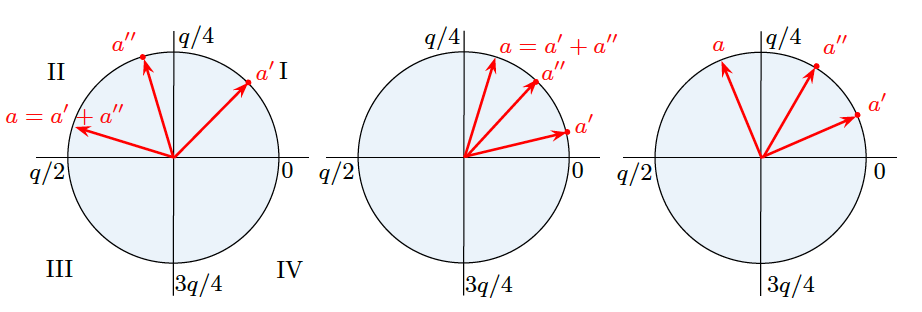
\includegraphics[width=\textwidth]{maskedDecoder_1.png}
	\caption{The basic idea of our masked decoder. The circle represents elements in \(\mathbb{Z}_q\). The first case shown allows us to conclude \(\textsc{Decode}(a)=1\), while we cannot make any guesses about the last two ones. \cite{maskedRing}}
	\label{maskedDecoder_1}
\end{figure}
Figure \ref{maskedDecoder_1} shows our example from above on the left. We can use this knowledge to state a total of four rules, the first of whom is taken from our example:
\begin{itemize}
\item \(0 < a' < q/4\), \(q/4 < a'' < q/2\) \(\implies\) \(a \in (q/4,3q/4)\) \(\implies\) \(\textsc{Decode}(a)=1\)
\item \(q/2 < a' < 3q/4\), \(3q/4 < a'' < q\) \(\implies\) \(a \in (q/4,3q/4)\) \(\implies\) \(\textsc{Decode}(a)=1\)
\item \(q/4 < a' < q/2\), \(q/2 < a'' < 3q/4\) \(\implies\) \(a \in (0,q/4) \cup (3q/4,q)\) \(\implies\) \(\textsc{Decode}(a)=0\)
\item \(3q/4 < a' < q\), \(0 < a'' < q/4\) \(\implies\) \(a \in (0,q/4) \cup (3q/4,q)\) \(\implies\) \(\textsc{Decode}(a)=0\)
\end{itemize}
With swapping \(a'\) and \(a''\) in the above rules, one can obtain another four rules. From the rules it follows that we only need to know the quadrant of each \(a'\) an \(a''\) to infer the output of \(\textsc{Decode}(a)\). However, this does not work for all cases, as Figure \ref{maskedDecoder_1} shows. We can actually only apply those rules in half of the possible cases.

So, what happens if our \((a', a'')\) does not match any rule? We simply need to refresh the splitting by computing \(a' = a' + \Delta_1\) and \(a'' = a'' - \Delta_1\) with \(\Delta_i \in \mathbb{Z}_q\). From \((a' + \Delta_1) + (a'' - \Delta_1) = a' + a'' = a\) it follow, that \(a\) stays unchanged by that refresh. Now that we have a fresh pair \((a',a'')\), we can again try to apply our rules from above. This process can be repeated until all shares have been decoded. Note, that a new \(\Delta_i\) should be chosen for each iteration. About half of the \(a',a''\) are decoded per iteration, so that the amount of decoded shares rises exponentially with the number of iterations. The authors of \cite{maskedRing} propose a number of \(N = 16\) iterations for a satisfactory result.
\begin{figure}[H]
	\centering
	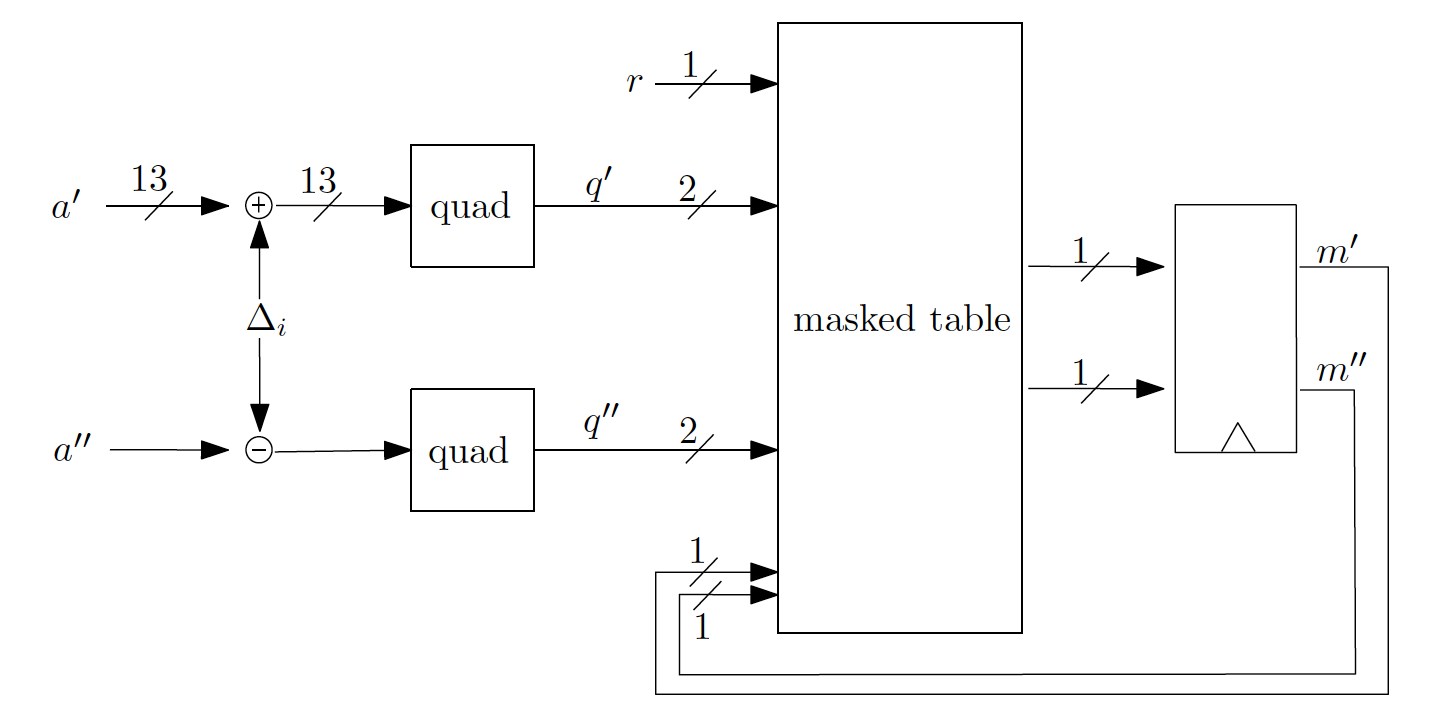
\includegraphics[width=0.7\textwidth]{maskedDecoder_2.png}
	\caption{Hardware implementation of the masked decoder. \cite{maskedRing}}
	\label{maskedDecoder_2}
\end{figure}
A possible hardware implementation of such a masked decoder is shown in Figure \ref{maskedDecoder_2}. The refreshing step is depicted on the left, using a different \(\Delta_i\) in each iteration. The quadrant function used in the next step simply takes a refreshed share \(a'\) or \(a''\) as an input and outputs two bits depending on the quadrant that the share belongs to. Next, a masked table is used to check the two bits against the rules we described above. Finally, the masked table function returns two one bit shares of the decoded message \(\textit{m}\). In our implementation the masked takes additional inputs, like a random bit \(r\) and the output of the last iteration \((m_{i-1}',m_{i-1}'')\). For more details on the masked table lookup, we would like to refer you to the paper of Oscar Reparaz et. al. \cite{maskedRing}.

%\subsection{Masked Table Lookup}
%Wenn noch Text fehlt, wird das hier eingefügt

\section{Evaluation}
Starting with efficiency, Reparaz et. al. showed that this implementation is at least 1.9x times better on a Virtex-2 FPGA than an unprotected high-speed elliptic curve scalar multiplier architecture introduced in \cite{Rebeiro2012}.

Furthermore, as both, the \textit{\ac{LPR} \ac{ring-LWE}} encryption scheme and our masked decoder, are probabilistic, there will always be a chance for errors occurring during decoding. The global error rate of decoding rises significantly when using our masked decoder instead of a deterministic decoder. To offset this effect, we can adapt the number of iterations for the masked decoder. While for \(N=3\) iterations the global error rate is about \(49\) times higher than when using a deterministic decoder, \(N=16\) iterations yield a global error rate that is almost identical with the one of a deterministic decoder. Further improvement could be achieved by increasing the number of iterations again, but this would lead to a significantly higher cycle count and thus to a much more inefficient implementation.

For our evaluation in terms of side-channel attack soundness, we assume the attacker knows the details of our implementation and is aware of the rest of the key while guessing a subkey. Our evaluation will follow three steps: First, we perform a first-order key recovery attack with our source of randomness (\textit{\acs{PRNG}}) turned off. This attack will be successful, showing that our setting is correct. In the second step, we will turn on the PRNG and repeat the same attack, but it should not be successful in this case. Finally, we perform a second-order attack to confirm the correctness of the first two steps.
\begin{figure}[H]
	\centering
	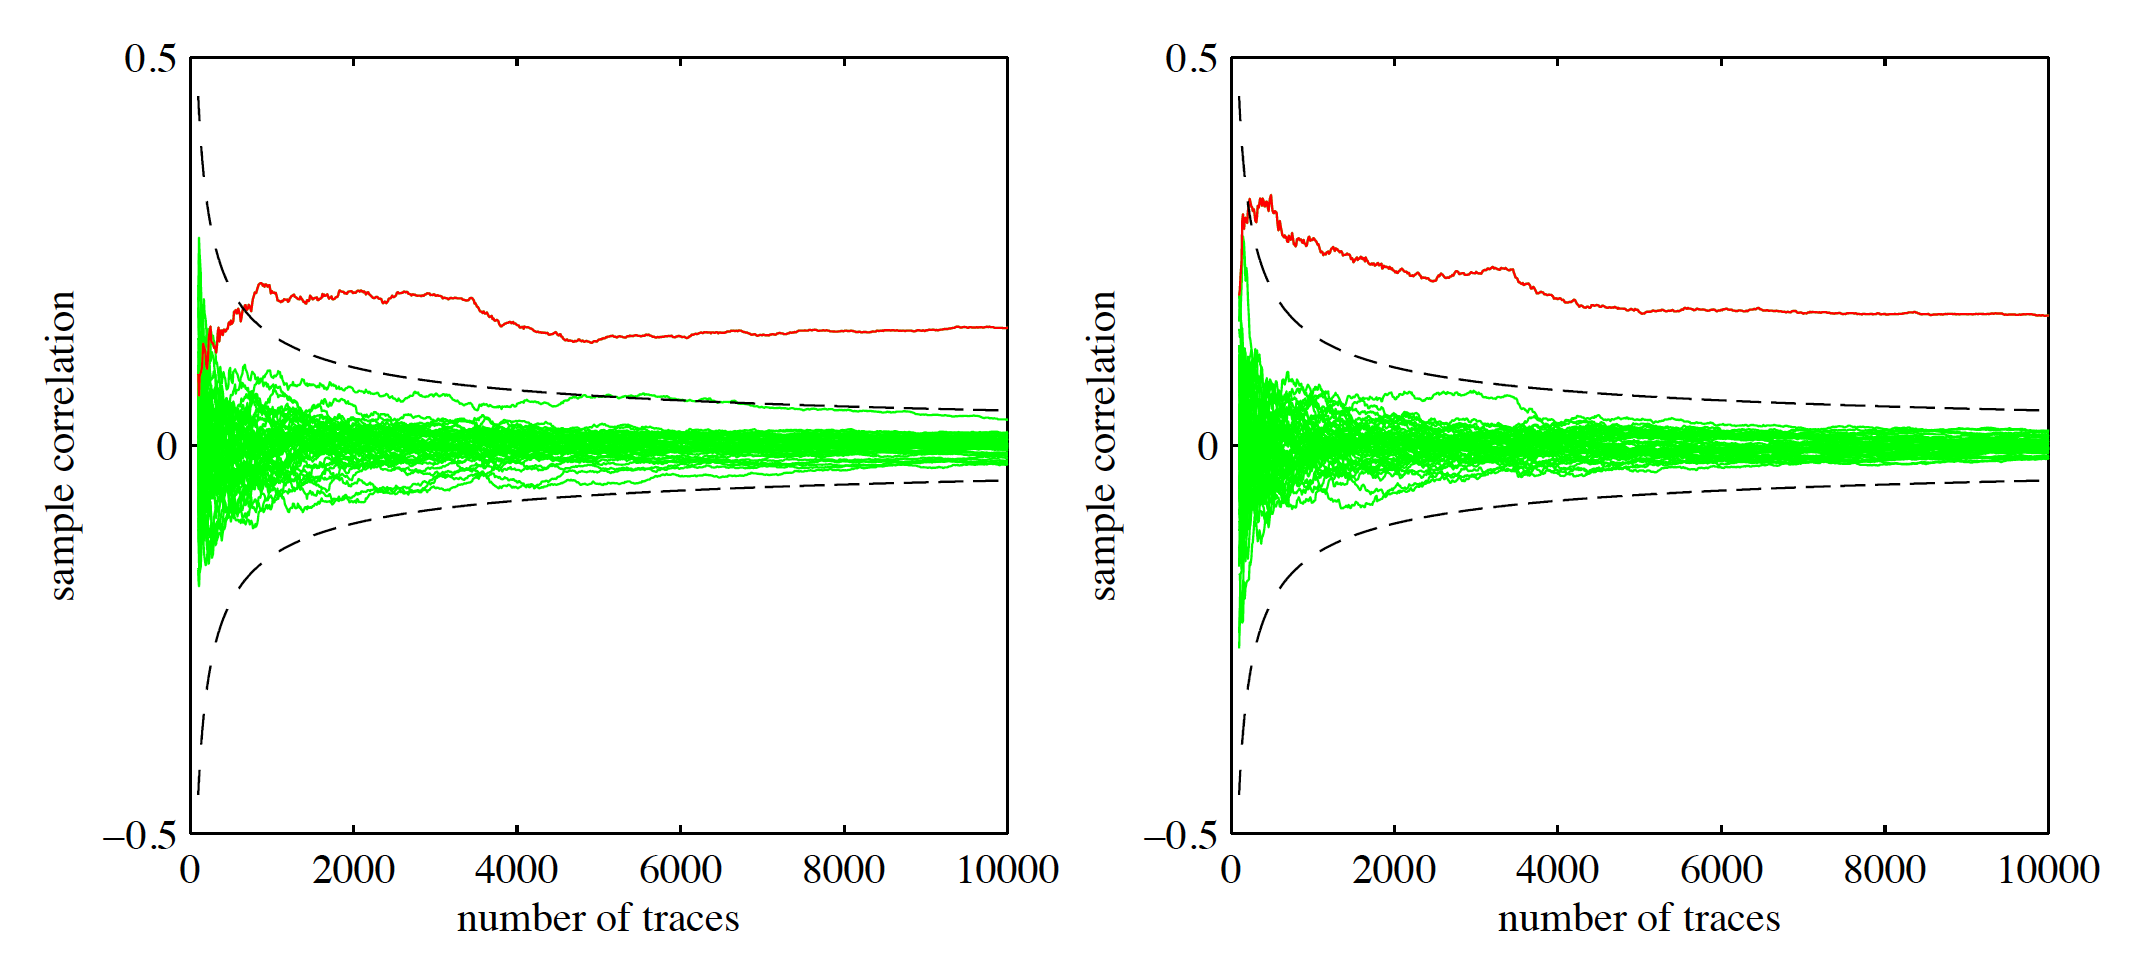
\includegraphics[width=0.7\textwidth]{dpa_1.png}
	\caption{\textit{\acs{PRNG}} is turned off. Graph shows the correlation coefficient increasing with the number of traces for the intermediates \(a'_0\) (left) and \(a''_0\) (right). The correct subkey is shown in red, all other guesses in green. \cite{maskedRing}}
	\label{dpa_1}
\end{figure}
For each of those steps, four different points that cover all relevant steps of the algorithm have been tested. The targets are \(a'_0\), \(a''_0\), the first input to the masked decoder and the first output bit. Pearson's correlation coefficient has been used to compare our guesses with real measurements \cite{Brier2004}.

\textbf{\textit{\acs{PRNG}} off:} When the \textit{\ac{PRNG}} is turned off, sharing of \(\textbf{s}\) in \(\textbf{s}'\) and \(\textbf{s}''\) is deterministic. This translates to the masking being turned off. Figure \ref{dpa_1} shows the correlation coefficient evolving with the number of traces. The attack seems to be successful starting at about a hundred traces.
\begin{figure}[H]
	\centering
	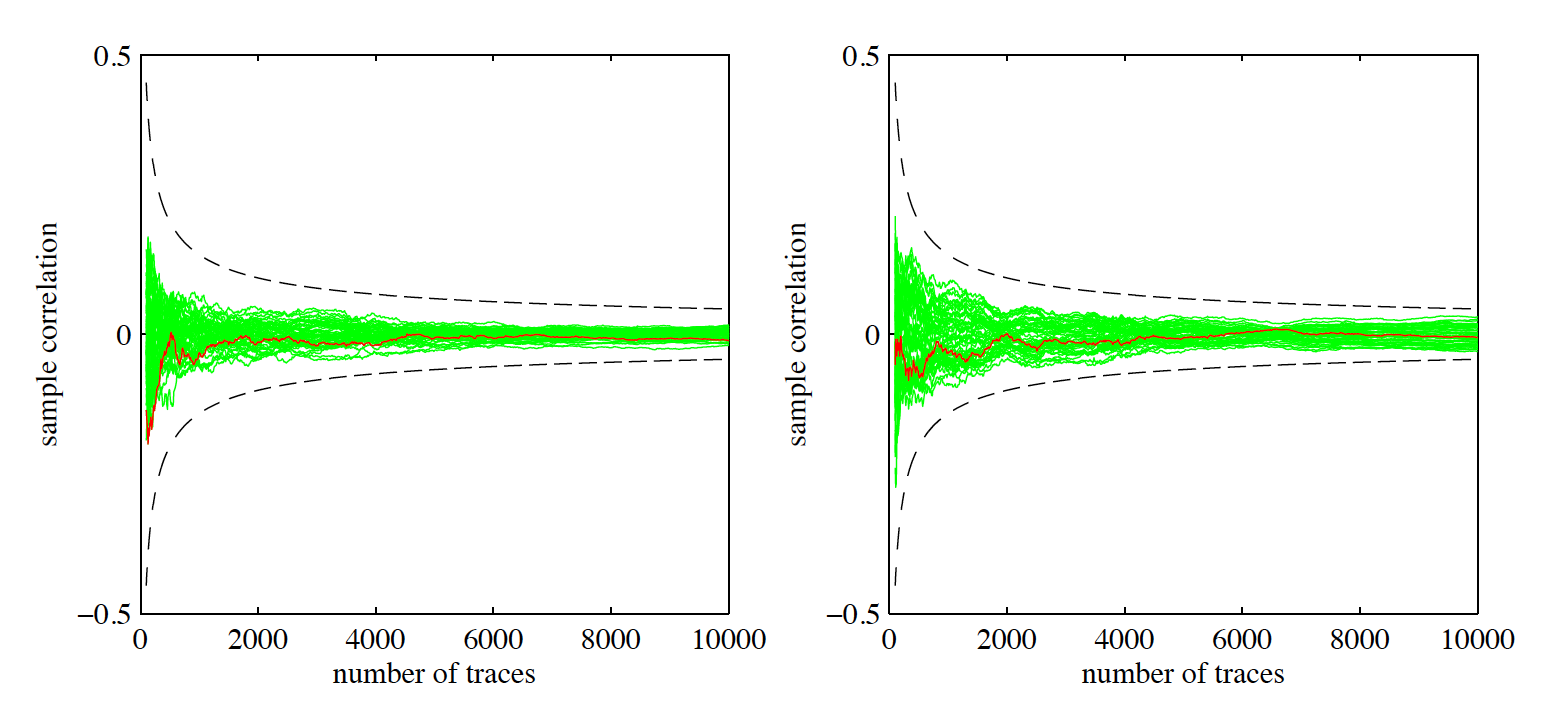
\includegraphics[width=0.7\textwidth]{dpa_2.png}
	\caption{Same as Figure \ref{dpa_1}, but with the \textit{\acs{PRNG}} turned on. It is no longer possible to identify the correct subkey within all guesses, meaning that the masking is successful. \cite{maskedRing}}
	\label{dpa_2}
\end{figure}

\textbf{\acs{PRNG} on:} When the \textit{\acs{PRNG}} is turned on, the masking is effective. As we can see in Figure \ref{dpa_2}, the correct subkey can no longer be distinguished from all the other guesses, not even with an enormous amount of traces. This is what an attacker would see when conducting an first-order \textit{\ac{DPA}} on our masking scheme.
\begin{figure}[H]
	\centering
	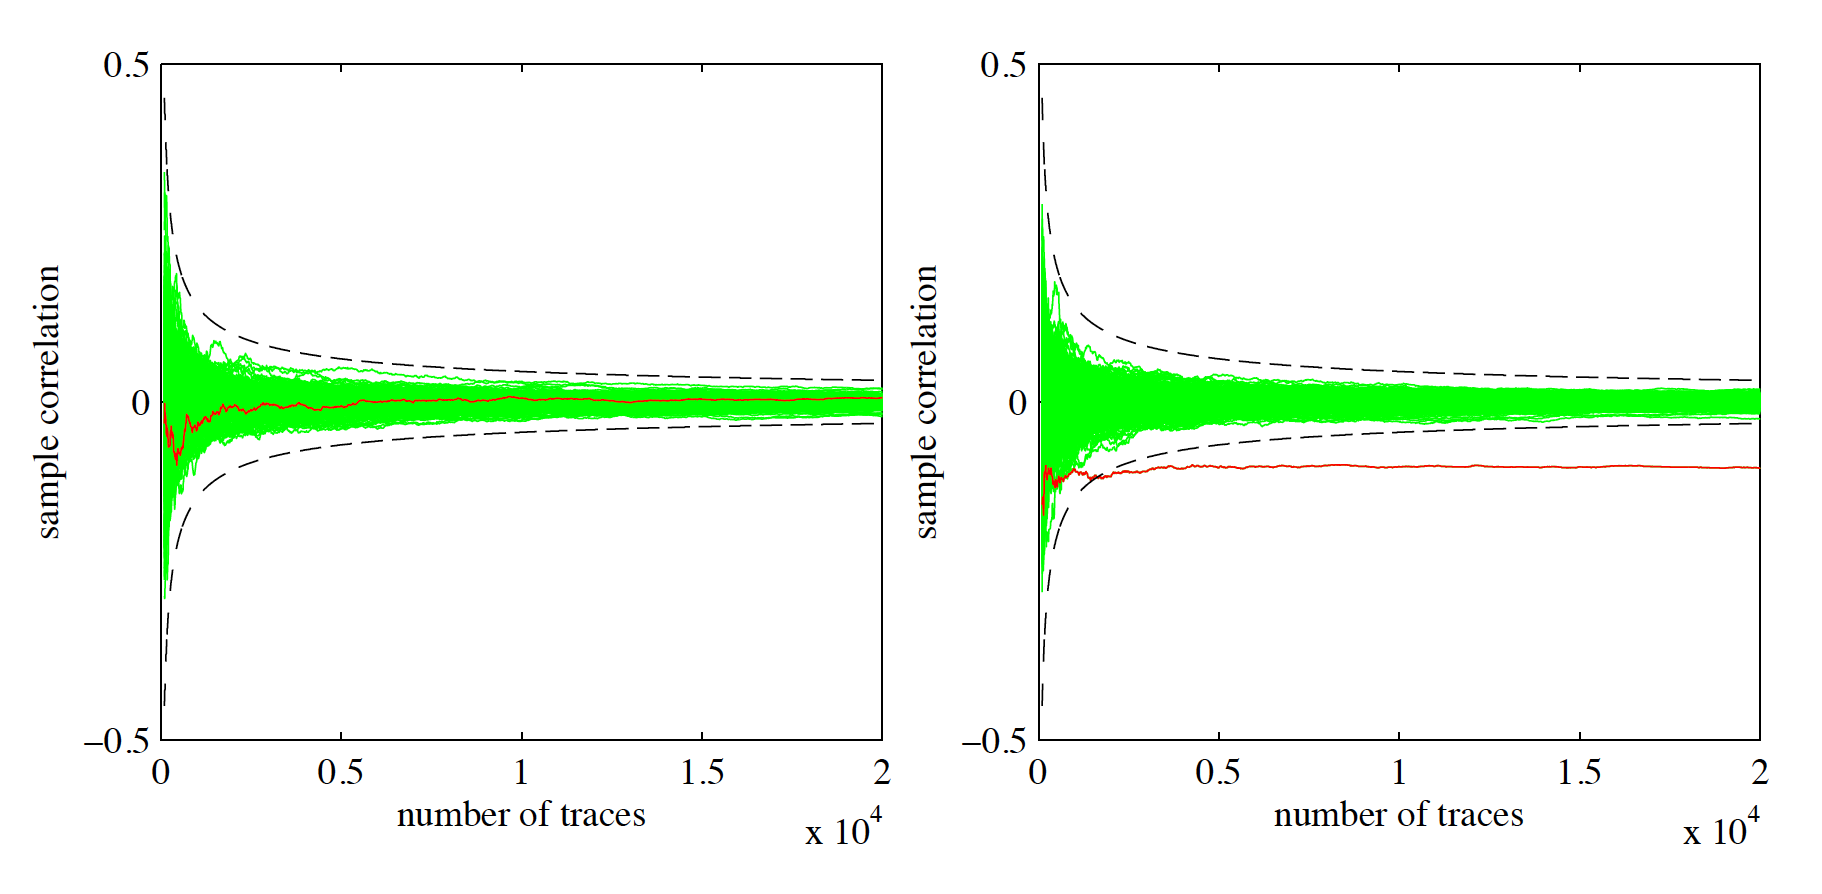
\includegraphics[width=0.7\textwidth]{dpa_3.png}
	\caption{On the left is the correlation for an increasing number of traces of a first-order attack with masking turned on. On the right we can see a successful second-order attack on our decoding scheme with masking turned on. \cite{maskedRing}}
	\label{dpa_3}
\end{figure}

\textbf{Second-Order Attack:} To confirm that we have used a sufficient number of traces in the first two steps, we perform a second-order attack on our masking scheme. In Figure \ref{dpa_3} we can see, that the second-order attack starts to be successful at around 2000 traces. From this we conclude, that we carried out the first-order attack on the activated masking scheme correctly, as we are already successful with 2000 traces. We stress that an attacker would need a significantly higher number of traces and computations in reality, as we used a pretty friendly setting for our scenario.